% Created 2023-05-15 Mon 12:26
% Intended LaTeX compiler: pdflatex
\documentclass[11pt]{article}
\usepackage[utf8]{inputenc}
\usepackage[T1]{fontenc}
\usepackage{graphicx}
\usepackage{grffile}
\usepackage{longtable}
\usepackage{wrapfig}
\usepackage{rotating}
\usepackage[normalem]{ulem}
\usepackage{amsmath}
\usepackage{textcomp}
\usepackage{amssymb}
\usepackage{capt-of}
\usepackage{hyperref}
\author{eric}
\date{\today}
\title{}
\hypersetup{
 pdfauthor={eric},
 pdftitle={},
 pdfkeywords={},
 pdfsubject={},
 pdfcreator={Emacs 27.1 (Org mode 9.2.6)}, 
 pdflang={English}}
\begin{document}

\noindent Aquí las ``predicciones'' reversas de 1988 a partir de 5 elecciones subsecuentes con supuesto de linealidad. Sin log-ratios del voto ni ruido estocástico, la estimación para un municipio \(u\) se vería así:

\begin{center}
\begin{tabular}{rrr}
\(t\) & \(v.pan_u\) & \(\hat{v.pan_u}\)\\
\hline
1988 & -- & .08\\
1991 & .10 & \\
1994 & .12 & \\
1997 & .14 & \\
2000 & .16 & \\
2003 & .18 & \\
\end{tabular}
\end{center}

\noindent \(v.pan_{u,t} = \beta_0 + \beta_1 t, t \in (1991,1994,1997,2000,2003)}\)

\noindent \(\hat{\beta_0}=-13.17\bar{3}\)

\noindent \(\hat{\beta_1}=.00\bar{6}\)

\noindent \(\therefore \hat{v.pan}_{u,1988} = \hat{\beta_0} + \hat{\beta_1} \times 1988 = .08\)

\bigskip Anexo predicciones de voto para diputados federales en distritos y municipios. Los municipios son unidades preferibles. Pero no tengo resultados 1988 para ese nivel y, sin esto, imposible contrastar predicciones lineales con los reportes oficiales. (¿Tienes resultados 1988 a nivel municipio?) 

Los plots siguientes usan distritos como unidad de observación/predicción. El eje Y es la diferencia entre el voto distrital y su predicción lineal (los residuales de las ecuaciones de arriba). El eje X estima los priistas \emph{core voters} en el distrito (la \(\alpha\)\textsubscript{PRI} de Federico, Alberto y Bea). La línea negra resume la nube de residuales.

\begin{center}
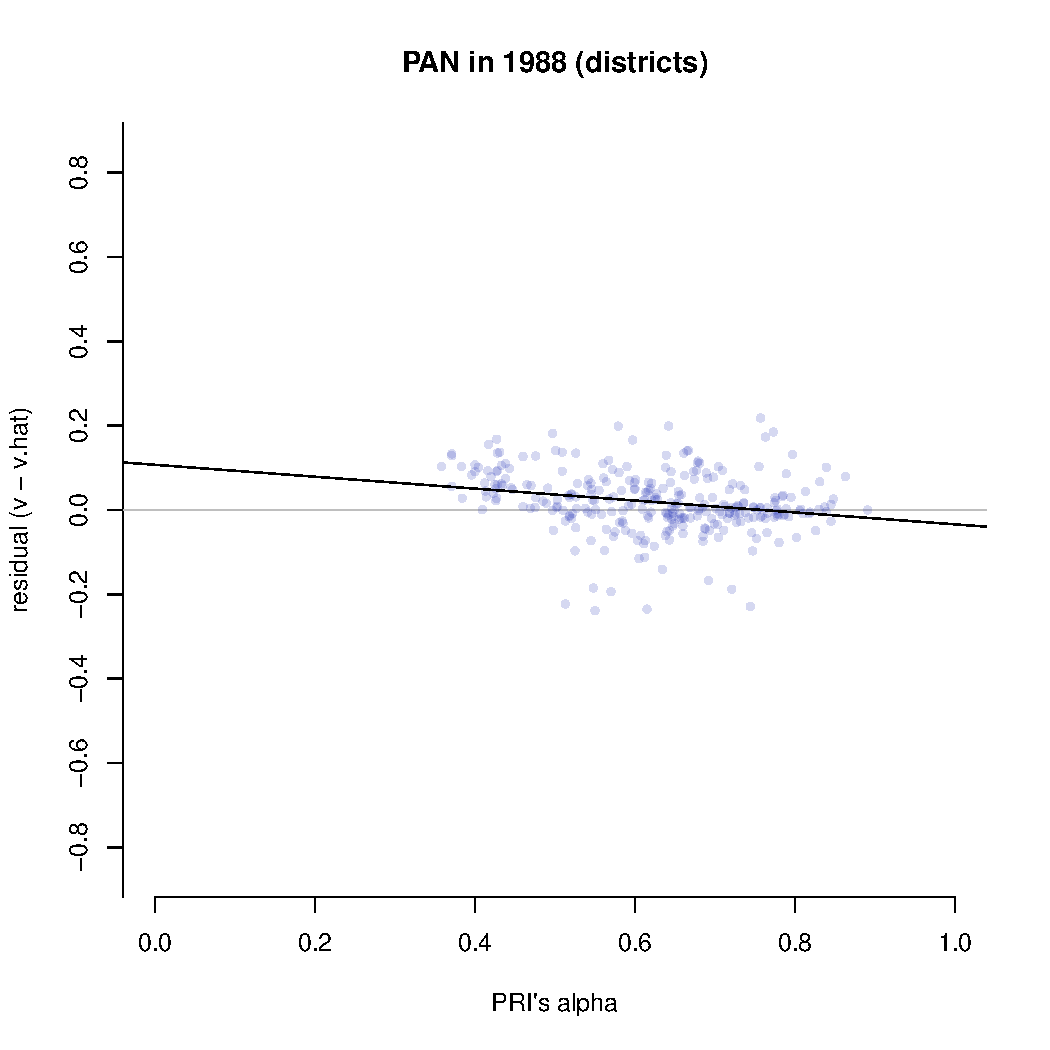
\includegraphics[width=200px]{./PAN1988alphaPRI.pdf}
\end{center}
\begin{center}
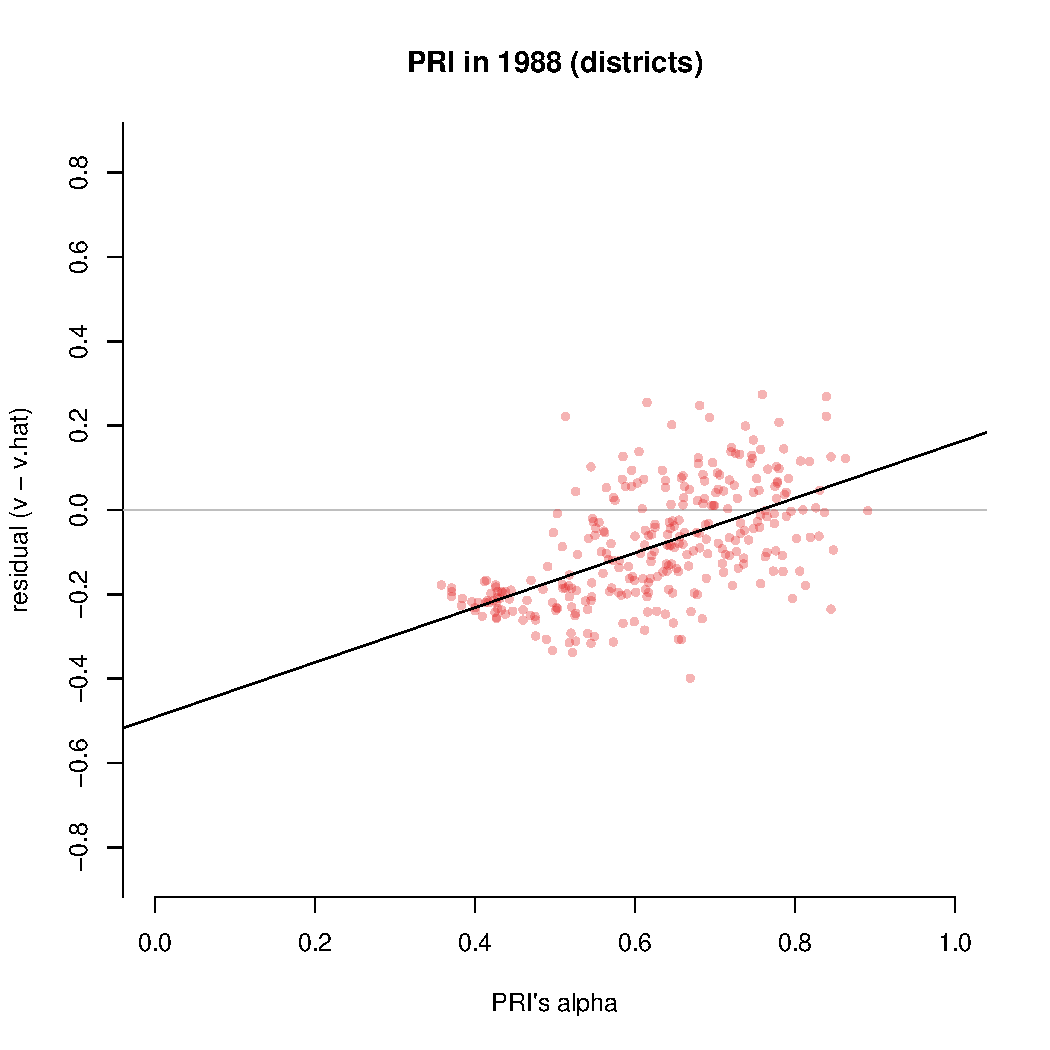
\includegraphics[width=200px]{./PRI1988alphaPRI.pdf}
\end{center}
\begin{center}
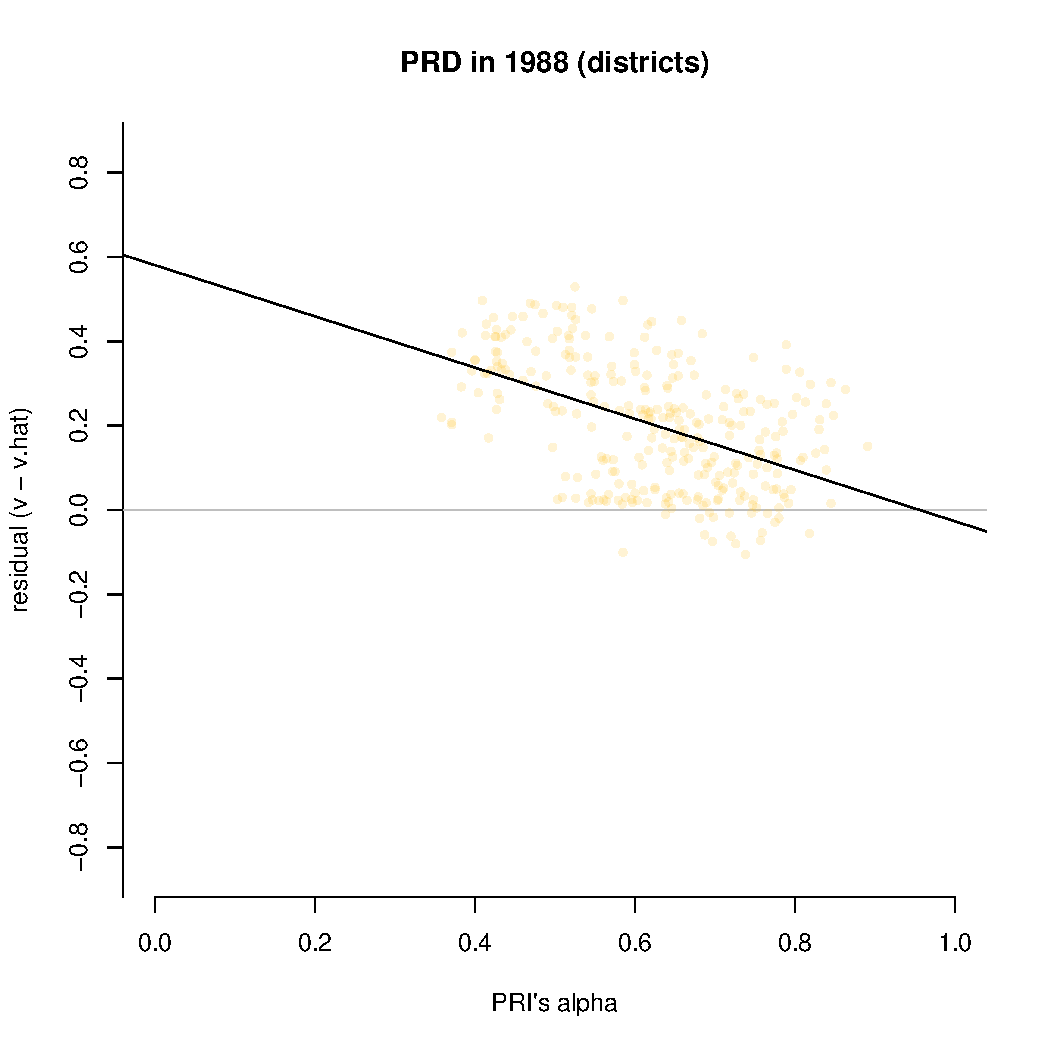
\includegraphics[width=200px]{./PRD1988alphaPRI.pdf}
\end{center}

En 1988 el PAN tuvo un desempeño más o menos en línea con la predicción autorregresiva lineal. El del PRI, en cambio, fue bien heterogéneo: 20 puntos por debajo de la predicción en sus peores distritos, tablas en sus mejores. La izquierda fue la imagen simétrica, 40 puntos arriba de pronóstico en los distritos menos priistas. La pendiente resumen pronunciada podría resultar del fraude---votos artificiales en distritos más priistas. Pero también podría ser que el segmento hegemónico del PRI aguantó el desprendimiento. 

Tengo reportes municipales para 1991. Muestran la recuperación priista con grano más fino. La pendiente resumen es menos empinada. 

\begin{center}
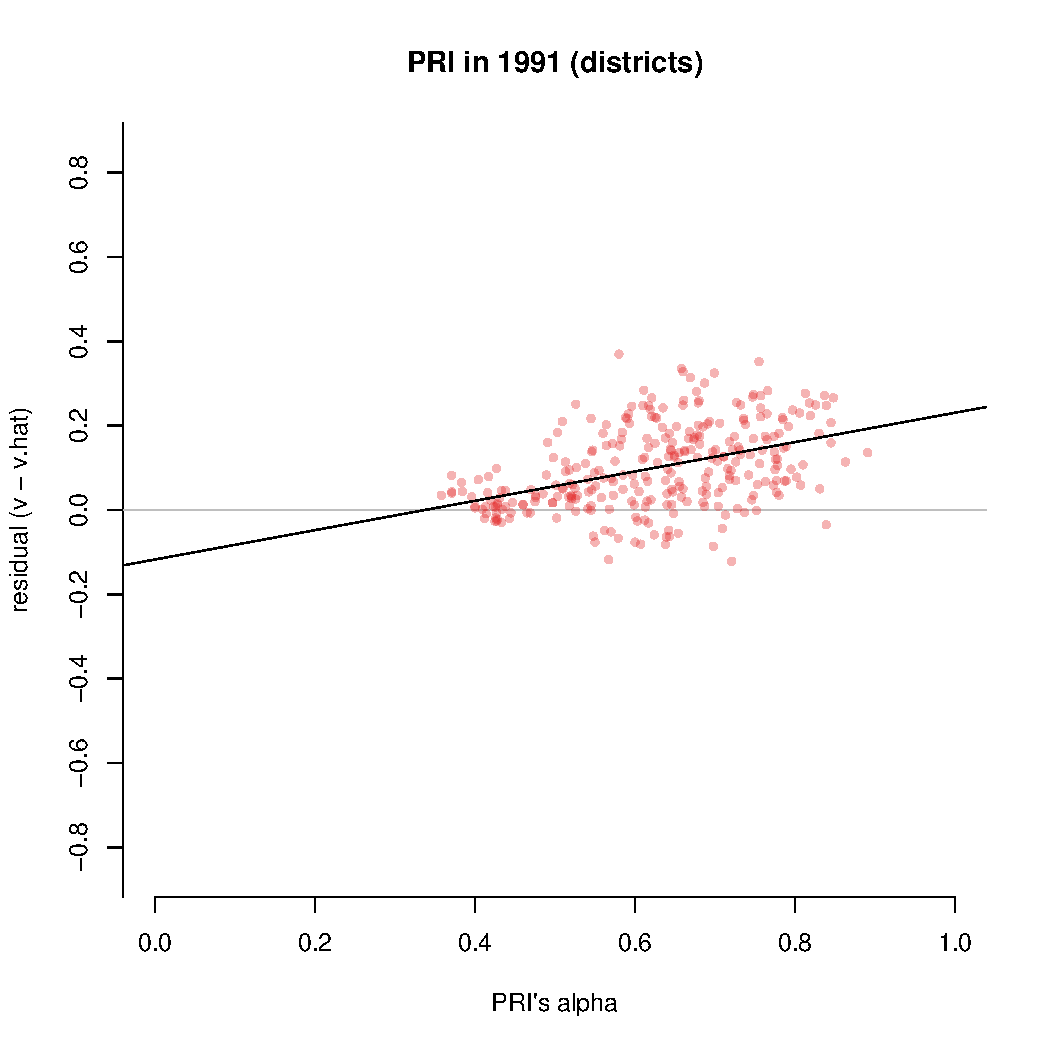
\includegraphics[width=200px]{./PRI1991alphaPRI.pdf}
\end{center}
\begin{center}
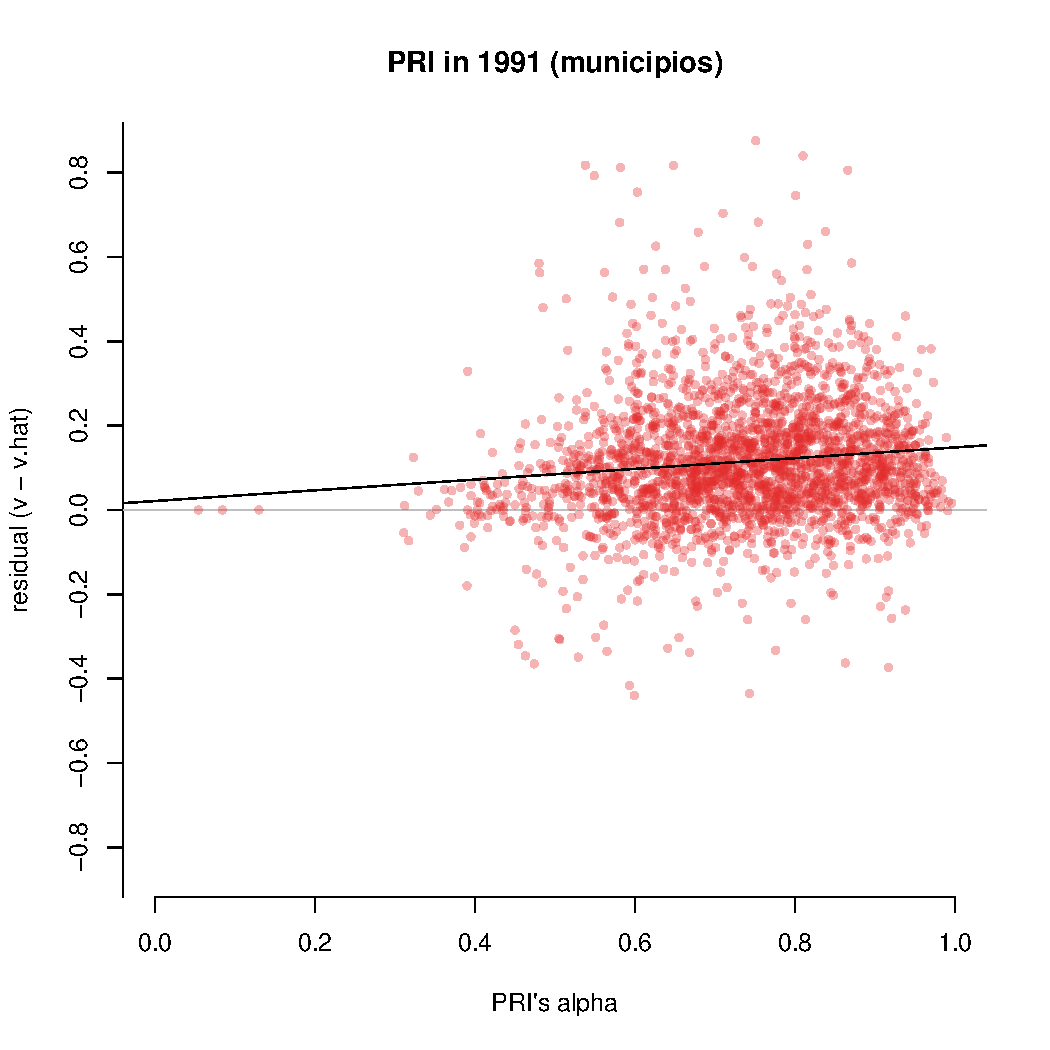
\includegraphics[width=200px]{./PRI1991alphaPRI.mun.pdf}
\end{center}

Cuando puedas, compara estas predicciones 1988 de serie de tiempo pura con tu predicción geográfica-temporal. A ver si arrojan algo de luz sobre esta cuestión.

Saludos, 

--e
\end{document}
